\documentclass[a4paper,twoside,11pt]{article}
\usepackage{a4wide,graphicx,subfigure,fancyhdr,amsmath,amssymb,algpseudocode,enumerate,hyperref, float}
\usepackage[english]{babel}
\numberwithin{equation}{section}

%----------------------- Macros and Definitions --------------------------

\setlength\headheight{20pt}
\addtolength\topmargin{-10pt}
\addtolength\footskip{20pt}

\newcommand{\N}{\mathbb{N}}
\newcommand{\ch}{\mathcal{CH}}

\fancypagestyle{plain}{%
\fancyhf{}
\fancyhead[LO,RE]{\sffamily\bfseries\large}
\fancyhead[RO,LE]{\sffamily\bfseries\large }
\fancyfoot[LO,RE]{\sffamily\bfseries\large }
\fancyfoot[RO,LE]{\sffamily\bfseries\thepage}
\renewcommand{\headrulewidth}{0pt}
\renewcommand{\footrulewidth}{0pt}
}

\pagestyle{fancy}
\fancyhf{}
\fancyhead[RO,LE]{\sffamily\bfseries\large 2IV05}
\fancyhead[LO,RE]{\sffamily\bfseries\large Project Proposal}
\fancyfoot[LO,RE]{\sffamily\bfseries\large }
\fancyfoot[RO,LE]{\sffamily\bfseries\thepage}
\renewcommand{\headrulewidth}{1pt}
\renewcommand{\footrulewidth}{0pt}
\newcommand{\name}{Bridge builder 3D}

%-------------------------------- Title ----------------------------------

\title{\vspace{-\baselineskip}\sffamily\bfseries 2IV05 - Bridge Builder}

\author{
Nicky Advokaat - 0740567 - {\tt n.advokaat@student.tue.nl} \\
Bart Wezel - 0740608 - {\tt b.j.p.a.v.wezel@student.tue.nl}\\
}

\date{3\textsuperscript{rd} quartile, 2014}

%--------------------------------- Text ----------------------------------

\begin{document}
\maketitle
\thispagestyle{empty}
\begin{abstract}
This report is a concept version describing our project  for the course 2IV05 Additional Component Computer Graphics.
\end{abstract}

\section{Introduction}
For our project we chose to do the geometric modeling assignment, for which the description reads:\\
\\
\textit{Make a geometry editor where the geometry is based on stacking simple building blocks. The editor should allow for efficient construction of complex scenes.}\\
\\
Instead of just constructing meaningless structures, we wanted to stimulate the user to build something meaningful. This inspired us to create \name, a game in which the player must construct a bridge over a cliff such that a train can pass over it. The bridge is constructed from a number of simple building blocks. The difficult part is that physical effects are applied on the bridge, such as gravity on the weight of the building blocks, the maximum force that can be applied on a block before it breaks, and the weight of the train riding over the bridge. Altogether, these effects might cause the bridge to collapse, so the goal is to build a well designed bridge that can withstand these effects so that the train may safely pass.

\section{Requirements}


\section{Analysis}
In this section we will describe the problems we will have to deal with to create \name. These problems can be roughly divided between: The physics of the bridge builder, the collapsing of the bridge and the interface of the bridge builder.
\subsection{Physics}
The problem with the physics is that we have to determine whether the bridge will collapse or not. This depends on the gravity and on the upward force. We can simply compute the gravity by taking the sum of the mass of each building block. The upward force is determined by pulling robes, and blocks that are build on land.  If we could keep it very simple: if the upward force is bigger than the gravity on the bridge, the bridge won't collapse. We will also have to deal with other factors. If all upward forces are at one side of the bridge, the bridge should collapse too. 
\subsection{Collapsing of the Bridge}
Visualizing the collapsing of the bridge is very difficult and depends a bit on the physics. Some buiding blocks fall faster and some could break. Most building blocks will rotate and there will be a lot of collisionss between the building blocks. We also have to visualize how the train falls down, and determine if it stays intact or some wagons break off. There could also be some special effect like smoke and fire. 
\subsection{Interface}
There are some problems that have to be fixed, to make the interface simple and easy to use. The action of connecting two building blocks should be easy, so the user does not have to click the exact pixel to make the intended connection. \\
It should be easy for the user to rotate the building blocks in the correct direction. \\


\section{Solution}
In this section we will describe the solutions to the problems. This are the problems we will have to deal with: The physics of the bridge builder, the collapsing of the bridge and  the interface of the bridge builder.
\subsection{Physics}
We will use the physics engine in JMonkeyengine to keep track of the weight, gravity, location and maybe tractive force of each building blocks. This will make it easier to write an algorithm that decides when the bridge will break that also depends on the connections between the building blocks. We will try for each building blocks what mass and tractive force is most realistic and we will have to find a realistic weight for the train. 
\subsection{Collapsing of the Bridge}
JMonkeyEnginge handles collisions between building blocks by looking at the weight and gravity on each building block and this will result in a realistic collapsing bridge. However we still have to compute whether a building block breaks and we still have to visualize some special effects like smoke or fire.
\subsection{Interface}
We decided to keep the interface very simple. The current interface looks like \ref{fig:gui}. In this interface only 2 building blocks are available, but we hope to get some more. There are some simple buttons. The two building blocks, the undo button and the play button for letting the train ride over the bridge. By pressing the letter matched to the button, will result in that action too.
\begin{figure}[H]
    \centering
    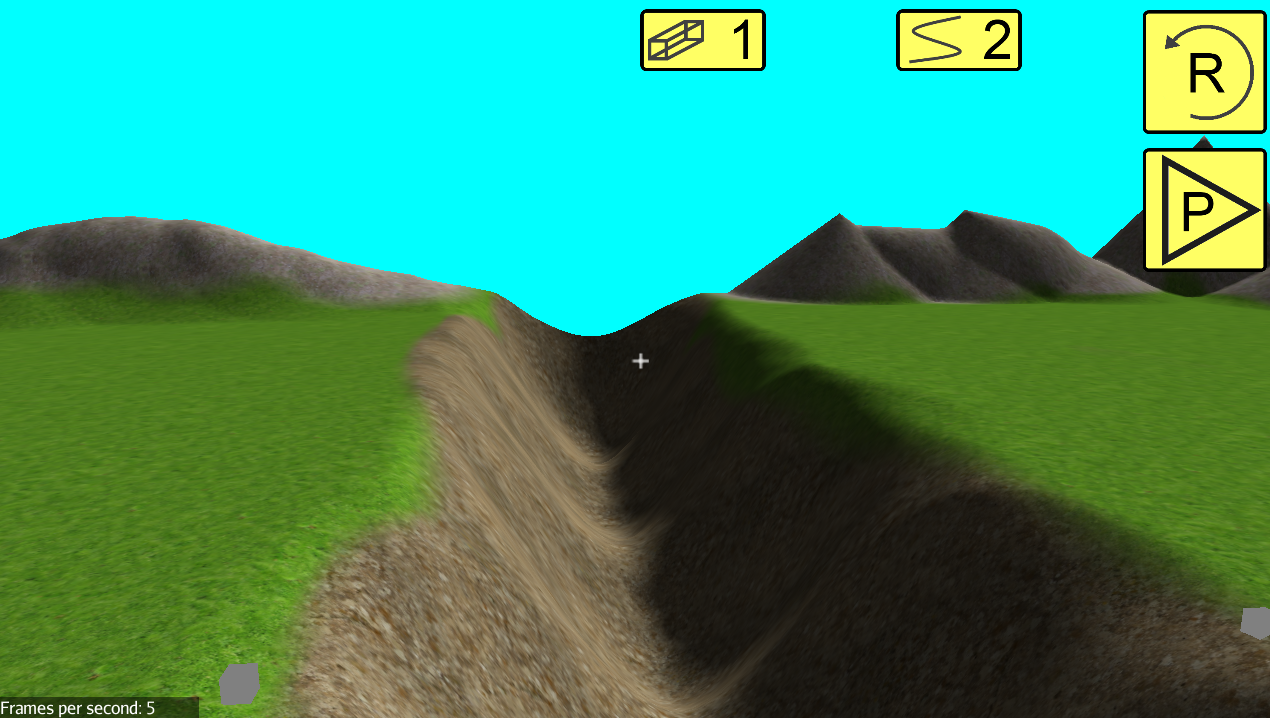
\includegraphics[width=0.8\textwidth]{screenshots/GUI.png}
    \caption{Current interface}
    \label{fig:gui}
\end{figure}
The user can click on a building block to select this building block. The selected building block will get another color as you can see in figure \ref{fig:bbs}. After that the user can select a point where he wants to connect the building block. This is shown in figure \ref{fig:scp}. When there is a connection point the user can select in which way the building block should be build. This is shown in figure \ref{fig:builded}.
\begin{figure}[H]
    \centering
    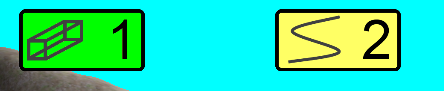
\includegraphics[width=0.4\textwidth]{screenshots/BuildingBlockSelected.png}
    \caption{Building block 1 is selected}
    \label{fig:bbs}
\end{figure}
\begin{figure}[H]
    \centering
    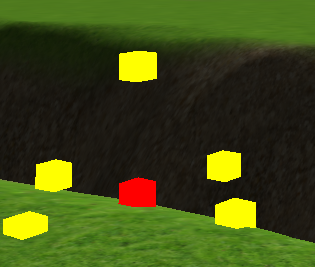
\includegraphics[width=0.4\textwidth]{screenshots/select.png}
    \caption{Selected connection point}
    \label{fig:scp}
\end{figure}
\begin{figure}[H]
    \centering
    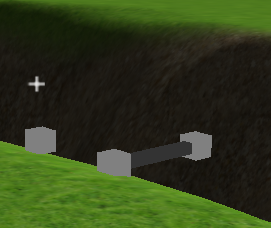
\includegraphics[width=0.4\textwidth]{screenshots/Builded.png}
    \caption{Building block is build}
    \label{fig:builded}
\end{figure}

\section{Motivation}


\section{Discussion of literature}


\section{Results and Evaluation}
\subsection{Results}
\subsubsection{Easy to use}
We wanted to make it easier for users  to build their bridge, so they can spend more time on thinking about the bridge and less time about clicking on the screen for each building block.  To make this possible we added two simple functions:\\
\begin{itemize}
\item \textbf{Connect to block:}
As you can see in figure x. It is possible to connect to other connection points directly, so that you do not have to build each block one by one. This will fasten the building, because usually you want to connect the two parts to make the bridge stronger. This is shown in \ref{fig:easyu1}a and \ref{fig:easyu2}a.
\item \textbf{Build multiple blocks in one direction:}
You can build multiple blocks in one direction in one click. This can help the user to make a straight bridge a lot faster. This is shown in \ref{fig:easyu1}b and \ref{fig:easyu2}b.
\end{itemize}
\begin{figure}[H]
    \centering
    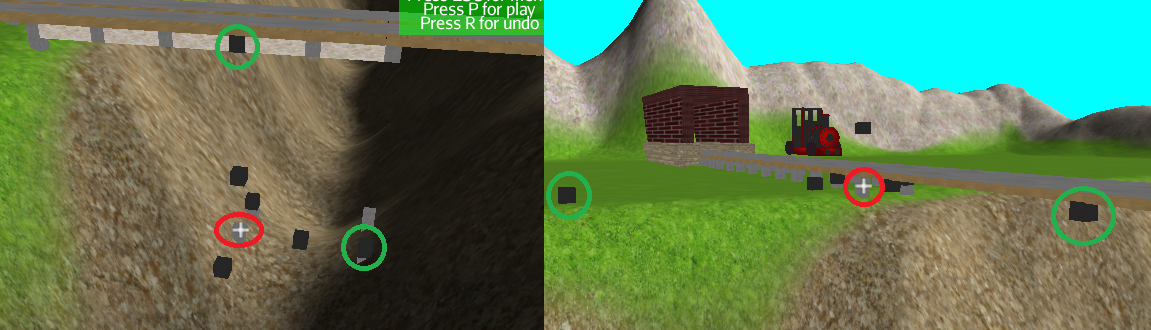
\includegraphics[width=1.0\textwidth]{screenshots/easyuse1.png}
    \caption{Empty world}
    \label{fig:easyu1}
\end{figure}
\begin{figure}[H]
    \centering
    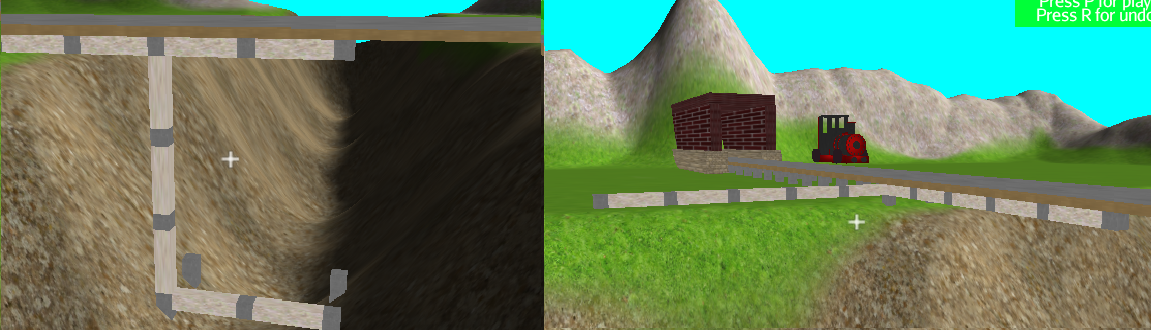
\includegraphics[width=1.0\textwidth]{screenshots/easyuse2.png}
    \caption{Empty world}
    \label{fig:easyu2}
\end{figure}
\subsubsection{Sample run}
When you start a new level, there will be an empty world as shown in \ref{fig:startup}. There will be connection points on both sides of the ravine. Depending on the level there could be more starting connection points. The user can start building a bridge by selecting a building block and a connection point. 
\begin{figure}[H]
    \centering
    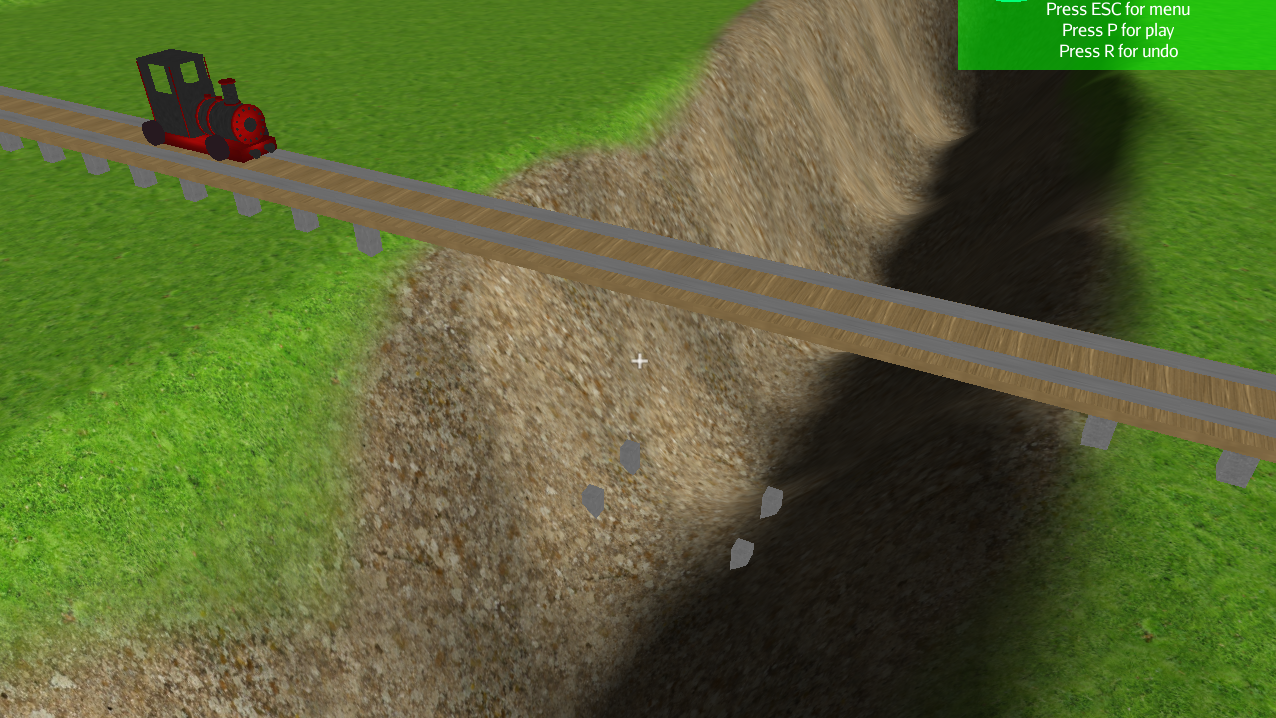
\includegraphics[width=0.8\textwidth]{screenshots/initial.png}
    \caption{Empty world}
    \label{fig:startup}
\end{figure}
After building a bridge the user can click on play, to start the simulation. The user cannot start the simulation if the 4 connection points are not connected. There has to be a connection between both sides of the ravine. A bridge built correctly is shown in \ref{fig:fullbridge}.
\begin{figure}[H]
    \centering
    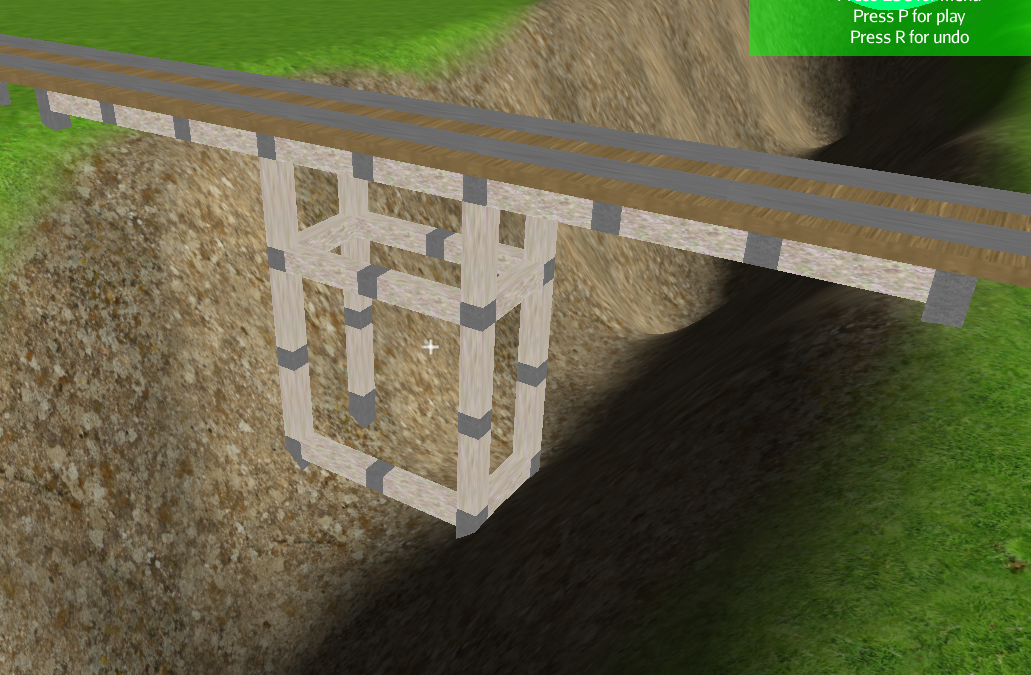
\includegraphics[width=0.8\textwidth]{screenshots/fullbridge.png}
    \caption{Bridge}
    \label{fig:fullbridge}
\end{figure}
When the user clicked on play and the bridge is built correctly, there will be a rail added automatically to the bridge. A train will ride over the bridge and the bridge will collapse or the train gets to the other side of the ravine safely as show in \ref{fig:full}
\begin{figure}[H]
    \centering
    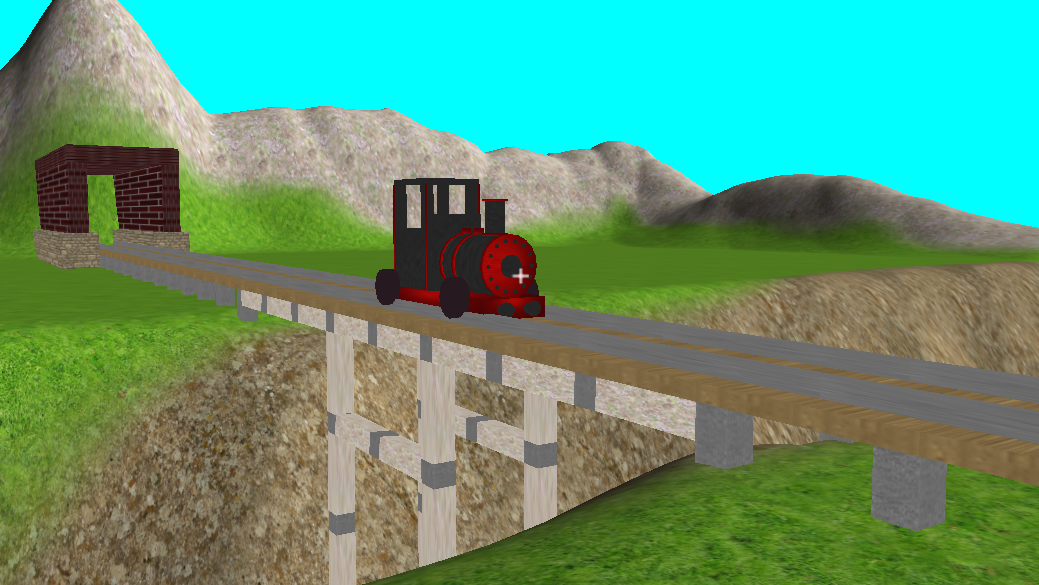
\includegraphics[width=0.8\textwidth]{screenshots/Drives.png}
    \caption{Succeed!}
    \label{fig:full}
\end{figure}
\subsection{Evaluation}
\subsubsection{Known limitations}
The rail for over the bridge is already drawn, which makes it harder to build under the bridge. This makes it also possible to build through the rails, which causes the physic engine to behave unrealistic. This is shown in \ref{fig:limit1}
\begin{figure}[H]
    \centering
    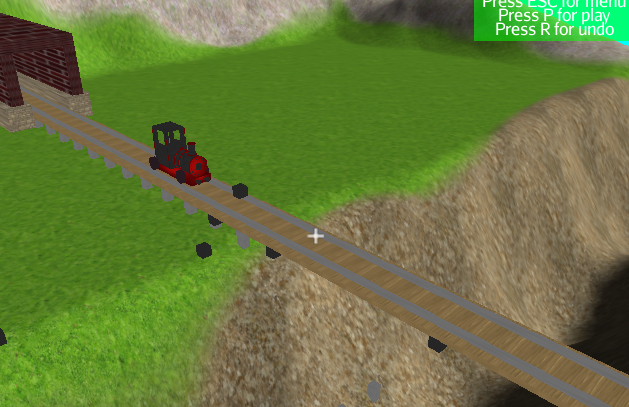
\includegraphics[width=0.4\textwidth]{screenshots/limit1.png}
    \caption{Building under the bridge is hard}
    \label{fig:limit1}
\end{figure}
When building, the block to which you want to build is black. This can be hard to see sometimes as the background can be a bit dark too. This is shown in \ref{fig:limit2}
\begin{figure}[H]
    \centering
    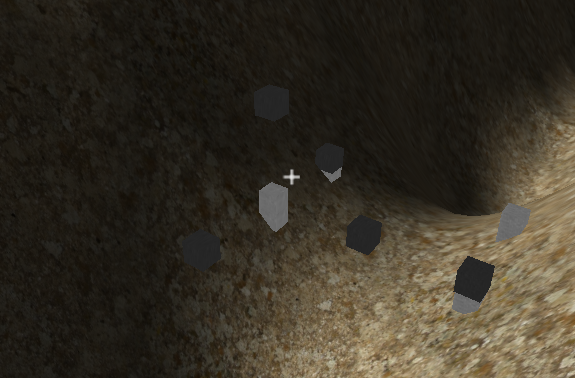
\includegraphics[width=0.4\textwidth]{screenshots/limi2.png}
    \caption{Sometimes connection points are hard to see, because of a dark background}
    \label{fig:limit2}
\end{figure}
There also other things that could be improved, but these are discussed in the next section.

\section{Conclusion and future work}
\subsection{Conclusion}
Developing a bridge builder was harder than we thought. During the process of making the bridge builder we encountered unexpected problems for which we had to find solutions. We were not able to implement all solutions, but in the future work we will describe how we would have implemented those solutions if we had more time. \\

The biggest problem was to make it easy to use, but at the same time giving a lot of freedom. The user is now unable to build in each direction he wants, but that makes it easier for him to connect the building blocks. If we did let him build in each direction, then it is easier to make small mistakes that can be troublesome at the other side of the bridge. When we started the project we thought our biggest problems would be the technical aspects of the game, but during the project we realized how hard it is to find the right balance between two different aspects of the game.  \\

We only had to make pretty small decisions, but we can imagine that the decisions at bigger project are much harder to make. Do they want better graphics, better performance or a combination that would increase the developing time? Do they want one long loading time or multiple smaller loading times? So compared to that trade-offs our decisions were relatively easy, so we can imagine that much more analysis has to done to make such important decisions at bigger projects.\\
\subsection{Future work}
\textbf{Different types of building blocks}\\
The most important thing that we would improve in a next version, is adding different kind of building blocks. This would greatly improve the different kinds of bridges that can be built with the bridge builder. When the user can build many different kinds of bridges, we can make the game more challenging for the user, because when there are only limited types of bridges that the user can build it is easier for the user to find the best type of bridge to build. \\
The problem we encountered with adding different kind of building blocks is that it is difficult to make them significantly different than the other building blocks. We had some ideas on how to make new building blocks different from others:\\
\begin{itemize}
\item A block that breaks in his own middle instead of at the connection points.
\item Give stronger blocks a lower score than weaker blocks.
\item Some building blocks will stretch out before they break
\item Some building blocks will break in the middle, while others should break at the connection points.
\end{itemize} 
\textbf{Limited building blocks per level}\\
Another feature that can be added is making some of the building blocks only available by a limited amount. This would limit the possible bridges that could be build, but at the same time make the game more challenging and lets users think better on how to use the building blocks instead of building a bridge with a large amount of blocks.  
It is not really hard to do it technically, but you have to look at each level to define what the limit of the blocks should be. If the limit of a level is too low it will discourage users to solve the level, but when the limit is too high there is no real challenge in solving the level.\\ \\
\textbf{Build in all directions}\\
It is only possible to build to the right, left, forward, backwards up or down. There could be made a lot of more different kind of bridges. An idea to build in every direction is to first show a horizontal circle where the users can decide in which direction he wants to build. Then another circle shows up so that the users choose if he wants to build up or down or just straight. 
\begin{figure}[H]
    \centering
    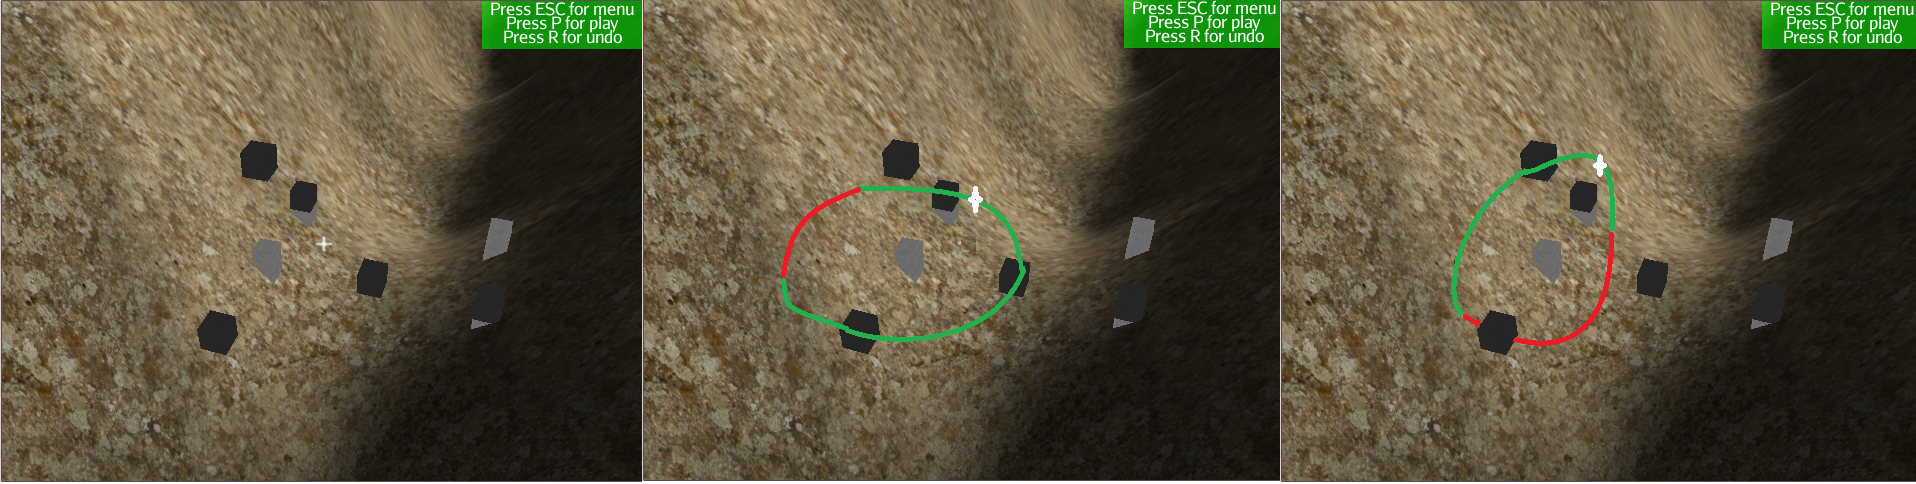
\includegraphics[width=0.8\textwidth]{screenshots/TwoClick.png}
    \caption{First screen is how it is now, second en third screen show the two clicks that have to be made to build in all directions}
    \label{fig:twoclick}
\end{figure}
This would cause some other problems. You have to check for collision, so that user does not build two building blocks that go through each other. You also have to make sure that the connection is still going good. If you are missing the other building block by a few pixels it should automatically connect to that building block, but maybe this is not always what you want.  \\ \\
\textbf{Save and load bridge}\\
A problem we encountered during testing the game is that when you build a bridge and you let the train drive over it and it collapses. You have to build the bridge again and cannot go back to the bridge before the collapsing. This really discourages the user when he spends a lot of time on a bridge that was almost perfect, but still collapsed then you have to build that bridge again to add some missing parts to make the bridge perfect. \\
The same problem occurs when you are working on a larger level and you have to go, and then you cannot continue working on that bridge when you get back. Unless you leave the program open.  This can be solved by an option to save and load your bridge. So you can save you bridge before you let a train drive over it and afterwards load that bridge so you can make it perfect.\\ \\
\textbf{More realistic world}\\
A more realistic world would make bridge builder more attractive to play. The world can be made more realistic by several improvements. 
There are not many environment details, like nature elements, buildings and humans. If these were added to Bridge Builder it would look even better.
The train could be made more realistic. This can be done by adding more details by the train, but it could also be done by loading a train model. There can be found multiple good looking train models on the internet that could be implemented in the project to get a better looking train.
The physics could be more realistic, by looking for a better balance between the mass of the train, the mass of the building blocks and the point at which building blocks fall apart. 


\end{document}
